\section{Aufbau}
\label{sec:aufbau}



        \begin{figure}
            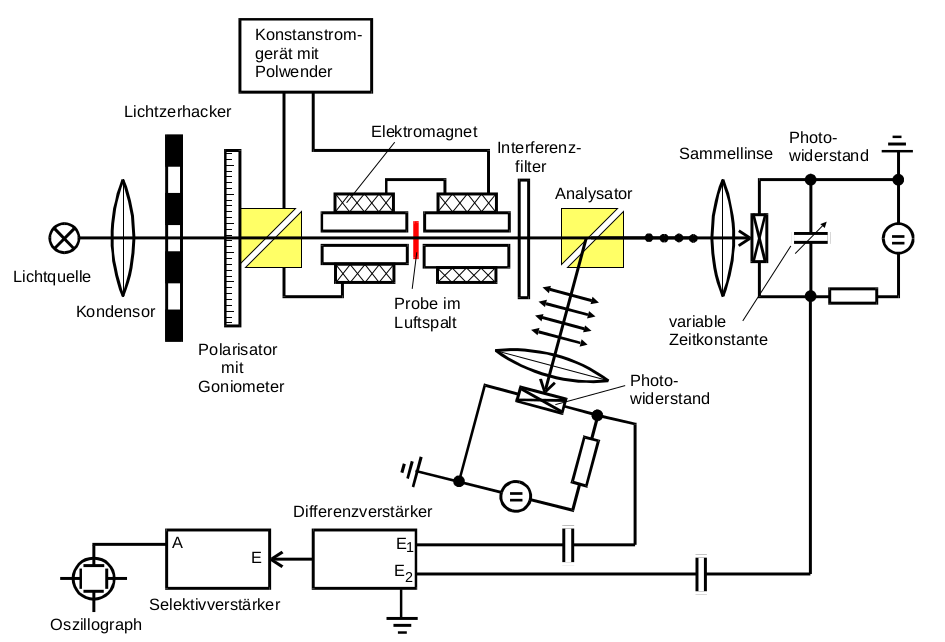
\includegraphics[width=0.7\textwidth]{aufbau.png}
            \centering
            \caption{Apparatur zur Messung der Faraday-Rotation \cite{alteanleitung}.}
            \label{fig:aufbau}
        \end{figure}

        Ein Bild des Aufbaus ist in der Abb. \ref{fig:aufbau} zu sehen. 
        Das für den Versuch verwendete, hauptsächlich infrarote, Licht 
        stammt aus einer Halogen-Lampe und durchläuft einen Kondensor,
        bevor es auf einen Lichtzerhacker trifft und in einzelne Pulse 
        geteilt wird. Danach trifft es auf ein Glan-Thompson-Prisma, 
        welches das Licht in s- und p-polarisiertes Licht aufteilt. 
        Nur einer dieser beiden Anteile wird später auf die Probe gelenkt,
        sodass das zur Messung verwendete Licht linear polarisiert ist.
        Die Probe kann in den Luftspalt von einem umpolbaren Elektromagneten
        eingesetzt werden, dessen Magnetfeldlinien parallel zum 
        einfallenden Licht sind. Hinter dem Magneten können Interferenzfilter 
        angebracht werden, welche je eine bestimmte Wellenlänge aus dem 
        Spektrum der Halogenlampe filtern. Dieses gefilterte Licht wird zur 
        sog. balancierten Detektion weitergeleitet. Dabei trifft es auf ein 
        weiteres Prisma, das wiederum das Licht in s- und p-polarisierten 
        Anteil aufteilt. Beide Anteile werden fokussiert und von je einem 
        Photowiderstand mit Innenwiderstand proportional zur Intensität aufgefangen.
        Die Photowiderstände geben ihr Intensitätssignal beide auf einen Differenzverstärker,
        welcher beide Intensitäten voneinander abzieht und das Ergebnis verstärkt.
        Die verstärkte Differenz wird durch einen Selektivverstärker geleitet, 
        der auf die Frequenz des Lichtzerhackers eingestellt ist und somit einen 
        Teil der Rauschspannungen der Photowiderstände herausfiltert. Das so gefilterte Signal
        wird von einem Oszilloskop abgebildet.
        

